%========================
\chapter{L'orienté objet}
%=========================

	\marginicon{objectif}
	Le cours de Java vous a présenté la programmation orienté objet.
	Dans ce chapitre, nous allons rapidement revoir ce sujet
	et présenter comment nous allons l'utiliser dans ce cours.
	Nous nous contenterons de parler d'\textit{encapsulation}. 
	Les autres piliers de l'orienté objet 
	(\textit{héritage} et \textit{polymorphisme}) 
	ne seront pas vus cette année.

%===================
\section{Motivation}
%====================

	Au cours de Java,
	vous avez vu que l'orienté objet permet de structurer une
	application en regroupant dans un même \emph{objet}
	des données et le code qui va manipuler ces données.
	
	Une autre façon de voir l'orienté objet
	est de constater qu'une classe permet de définir 
	un nouveau \emph{type de données}.
	La notion de \emph{structure} permet déjà cela mais de façon limitée
	car elle ne reprend que des données et pas du code.
	Avec l'orienté objet, 
	on dispose de méthodes définissant ce qu'on peut faire avec des données
	(les objets) de ce type.
	C'est ainsi que nous l'utiliserons pour définir les listes 
	dans un prochain chapitre.

	
%=======================================
\section{Illustration~: une durée}
%=======================================

	Voyons tout cela au travers d'un exemple complet.
	Il est parfois utile d'avoir à sa disposition un type
	de données permettant de représenter une durée.	
	Utiliser plusieurs entiers (un pour les heures, un autre pour les minutes,
	un autre encore pour les secondes) n'est pas pratique.
	Utiliser une structure est déjà mieux mais offre moins d'avantage
	que l'orienté objet.	
	Voyons comment définir ce nouveau type de données en orienté objet.
	
	\subsection{Ce que l’on veut vraiment}
	%=====================================
	
		Avant tout, il faut bien préciser ce que l’on veut décrire
		et bien faire la distinction entre un \emph{moment} et une \emph{durée}.
		L’«~heure~» est un concept multifacette. 
		Parle-t-on de l’heure comme moment dans la journée 
		ou de l’heure comme représentant une durée ? 
		Dans le premier cas, elle ne peut dépasser 24h 
		et la différence entre 2 heures n’a pas de sens 
		(ou plus précisément n’est pas une heure, mais une durée !).
		Ce que nous nous proposons de créer ici est une durée,
		correspondant au deuxième cas.
		Et pour être plus précis encore,
		nous allons nous limiter à une précision à la seconde près,
		pas plus%
		\footnote{%
			Ajouter plus de précision ne serait pas plus compliqué à faire.%
		}.
	
	\subsection{Le comportement (les méthodes)}
	%==========================================
	
		La première question à se poser est celle des services que l’on veut
		fournir, c’est-à-dire des méthodes publiques de la classe. On doit
		pouvoir \textit{construire} une durée. On doit pouvoir connaitre le
		nombre de jours, d’heures, minutes ou secondes correspondant à une durée. On doit
		pouvoir effectuer des calculs avec des durées (addition, soustraction).
		Enfin, on doit pouvoir comparer des durées. Arrêtons-nous là, mais en
		pratique, on pourrait trouver encore bon nombre d’autres méthodes qu’il
		serait intéressant de fournir. 
		
		Voici comment nous allons noter tout cela au cours d'algorithmique.
		
		\begin{LDA}
			\Class{Durée}
				%\Private
					%\LComment rien encore
				\Public
					\ConstrSign{Durée}{secondes~: entier}
					\ConstrSign{Durée}{heure, minute, seconde~: entiers}
					\Empty
					\MethodSign{getJour}{}{entier}
					\RComment nb de jours dans une durée
					\MethodSign{getHeure}{}{entier}
					\RComment entier entre 0 et 23 inclus
					\MethodSign{getMinute}{}{entier}
					\RComment entier entre 0 et 59 inclus
					\MethodSign{getSeconde}{}{entier}
					\RComment entier entre 0 et 59 inclus
					\Empty
					\MethodSign{getTotalHeures}{}{entier}
					\RComment Le nombre total d’heures
					\MethodSign{getTotalMinutes}{}{entier}
					\RComment Le nombre total de minutes
					\MethodSign{getTotalSecondes}{}{entier}
					\RComment Le nombre total de secondes
					\Empty
					\MethodSign{ajouter}{autreDurée~: Durée}{}
					\MethodSign{différence}{autreDurée~: Durée}{Durée}
					%\MethodSign{égale}{autreDurée~: Durée}{booléen}
					\MethodSign{plusPetit}{autreDurée~: Durée}{booléen}
			\EndClass
		\end{LDA}
		
		\marginicon{attention}
		\textbf{Quelques remarques}
		\begin{itemize}
			\item
				On a deux constructeurs, ce qui offre plus de souplesse pour initialiser un objet. 
				On parle de «\textbf{~surcharge~}» des constructeurs.
			\item
				Faisons bien la distinction entre les méthodes
				\lda{getXXX()} et \lda{getTotalXXX()}. Par
				exemple, la méthode \lda{getMinute()} retourne la valeur
				de la composante «~minutes~» dans une représentation HMS tandis que la
				méthode \lda{getTotalMinutes()} retourne le nombre total
				de minutes entières pour cette durée. Ex~: pour 1h23’12’’,
				\lda{getMinute()} retourne 23 et
				\lda{getTotalMinutes()} retourne 83. 
				Idem avec les heures et les secondes.
			\item 
				Les méthodes \lda{getTotalXXX()} retournent le nombre
				(toujours entier) de XXX contenus dans la durée. Exemple, avec la durée
				0h23’52’’, \lda{getTotalMinutes()}
				retourne 23 et pas 24 (autrement dit, il n’y a pas d’arrondi vers le
				haut).
			\item 
				Il n’y a pas de \textit{mutateur} (\lda{setXXX()}). 
				Ce qui signifie qu’on ne peut pas changer directement la valeur de l’objet
				après son initialisation. 
				Les seules modifications viendront de la méthode \lda{ajouter()}.
				On aurait pu définir des mutateurs mais nous
				n'avons pas jugé utile de le faire dans ce cas précis.
				Vous verrez dans le cours de Java des motivations à ce choix.
			\item 
				La méthode \lda{ajouter()} ne retourne rien. En effet,
				elle ajoute la durée à l’objet sur lequel est appelée la méthode. C’est
				un choix ; on aurait aussi pu dire que la méthode ne modifie pas
				l’objet mais en retourne un autre qui représente la somme. Dans ce cas,
				on l’aurait plutôt appelée «\lda{~plus( )}~».
			\item 
				La méthode \lda{différence()}, elle, renvoie toujours une
				durée (positive).
			\item 
				Nous ne définissons pas de méthode d'affichage
				similaire au \lda{toString()} qu'on retrouve en Java.
				L'affichage correct de l'information ne fait pas partie
				des préoccupations de ce cours.
				On supposera que "\lda{\K{afficher} objet}"
				affiche correctement les données associées à l'objet.
		\end{itemize}
	
	\subsection{La représentation de l'état (les attributs)}
	%=======================================================
	
		La question suivante est~: «~Comment représenter une durée en interne ?
		». Plusieurs possibilités existent. Par exemple~:	
		\begin{itemize}
			\item 
				via le nombre d’heures, de minutes et de secondes
			\item 
				via le nombre total de secondes
			\item 
				via une chaine, par exemple au format «~HH~:~MM~:~SS~» où HH pourrait
				éventuellement excéder 23.
		\end{itemize}
		
		Le premier choix semble le plus évident mais réfléchissons-y de plus
		près. D’une part, pourquoi se limiter aux heures. On pourrait
		introduire un champ ‘\lda{jour}’ (après tout on a bien
		une méthode \lda{getJour()}). 		
		Quel critère doit vraiment nous permettre de décider ? Il faut une
		représentation qui soit suffisante (tout est représenté) et qui
		permette d’écrire des méthodes lisibles et si possible efficaces
		(c'est-à-dire où le calcul est rapide). Selon ces
		critères, la deuxième représentation est de loin la meilleure. 
		
		Voilà comment nous indiquons les attributs d'une classe.
		
		\begin{LDA}
			\Class{Durée}
				\Private
					\Decl{totalSecondes}{entier}
				\Public
					\LComment Ici viennent les constructeurs et les méthodes
			\EndClass
		\end{LDA}
	
		Pour rappel de votre cours de langage,
		ce qui est privé n'est pas utilisable directement 
		par du code extérieur à la classe.
		Un code extérieur, manipulant des objets de cette classe,
		ne peut utiliser que ce qui est public.
		
	\subsection{L'implémentation}
	%============================
	
		On est à présent prêt pour écrire le code des méthodes. 
		Pour une meilleure lisibilité,
		nous gardons les signatures des méthodes dans la classe
		et nous détaillons leur contenu en dehors.
		Ce qui donne :
		
		\begin{LDA}
			\Class{Durée}
				\Private
					\Decl{totalSecondes}{entier}
				\Public
					\ConstrSign{Durée}{secondes~: entier}
					\ConstrSign{Durée}{heure, minute, seconde~: entiers}
					\Empty
					\MethodSign{getJour}{}{entier}
					\RComment nb de jours dans une durée
					\MethodSign{getHeure}{}{entier}
					\RComment entier entre 0 et 23 inclus
					\MethodSign{getMinute}{}{entier}
					\RComment entier entre 0 et 59 inclus
					\MethodSign{getSeconde}{}{entier}
					\RComment entier entre 0 et 59 inclus
					\Empty
					\MethodSign{getTotalHeures}{}{entier}
					\RComment Le nombre total d’heures
					\MethodSign{getTotalMinutes}{}{entier}
					\RComment Le nombre total de minutes
					\MethodSign{getTotalSecondes}{}{entier}
					\RComment Le nombre total de secondes
					\Empty
					\MethodSign{ajouter}{autreDurée~: Durée}{}
					\MethodSign{différence}{autreDurée~: Durée}{Durée}
					%\MethodSign{égale}{autreDurée~: Durée}{booléen}
					\MethodSign{plusPetit}{autreDurée~: Durée}{booléen}
			\EndClass
		\end{LDA}

		\begin{LDA}
			\Constr{Durée}{secondes~: entier}
				\If{secondes < 0}
					\Stmt \K{erreur} "paramètre négatif"%
					\footnote{%
						L'instruction \K{erreur} indique
						que l'algorithme ne peut pas poursuivre normalement.
						Il s'arrête avec un message d'erreur.
					}					
				\EndIf
				\Let totalSecondes \Gets secondes
			\EndConstr
		\Empty
			\Constr{Durée}{heure, minute, seconde~: entiers}
				\If{heure < 0 OU minute < 0 OU seconde < 0 OU minute>59 ou seconde>59}
					\Stmt \K{erreur} "un des paramètres est invalide"
				\EndIf
				\Let totalSecondes \Gets 3600*heure + 60*minute + seconde
			\EndConstr
		\Empty
			\LComment Retourne le nombre de jours dans une 
			représentation JJ/HH:MM:SS
			\Method{getJour}{}{entier}
				\Return totalSecondes DIV (3600*24)
			\EndMethod
		\Empty
			\LComment Retourne le nombre d'heures dans une 
			représentation JJ/HH:MM:SS
			\Method{getHeure}{}{entier}
				\LComment On doit enlever les jours éventuels
				\Return (totalSecondes DIV 3600) MOD 24
			\EndMethod
		\Empty
			\LComment Retourne le nombre de minutes dans une 
			représentation JJ/HH:MM:SS
			\Method{getMinute}{}{entier}
				\LComment On doit enlever les heures éventuelles
				\Return (totalSecondes DIV 60) MOD 60
			\EndMethod
		\Empty
			\LComment Retourne le nombre de secondes dans une 
			représentation JJ/HH:MM:SS
			\Method{getSeconde}{}{entier}
				\LComment On doit enlever les minutes éventuelles
				\Return totalSecondes  MOD 60
			\EndMethod
		\Empty
			\LComment Retourne le nombre entier d’heures complètes
			\Method{getTotalHeures}{}{entier}
				\Return totalSecondes DIV 3600
			\EndMethod
		\Empty
			\LComment Retourne le nombre entier de minutes complètes
			\Method{getTotalMinutes}{}{entier}
				\Return totalSecondes DIV 60
			\EndMethod
		\Empty
			\LComment Retourne le nombre entier de secondes complètes
			\Method{getTotalSecondes}{}{entier}
				\Return totalSecondes
			\EndMethod
		\Empty
			\Method{ajouter}{autreDurée~: Durée}{}
				\Let totalSecondes \Gets totalSecondes + autreDurée.getTotalSecondes()
			\EndMethod
		\Empty
			\Method{différence}{autreDurée~: Durée}{Durée}
				\Return \K{nouvelle} Durée(valeurAbsolue(totalSecondes - autreDurée.getTotalSecondes()))
			\EndMethod
		%\Empty
			%\Method{égale}{autreDurée~: Durée}{booléen}
				%\Return totalSecondes = autreDurée.getTotalSecondes()
			%\EndMethod
		\Empty
			\Method{plusPetit}{autreDurée~: Durée}{booléen}
				\Return totalSecondes < autreDurée.getTotalSecondes()
			\EndMethod
		\end{LDA}
	
	%=====================================
	\subsection{Utilisation}
	%=====================================

		Pour utiliser le nouveau type de donnée créé,
		il faut l'instancier, c'est-à-dire créer un nouvel objet de ce type.
		Nous allons utiliser le mot clé \K{nouveau}
		(ou \K{nouvelle} si vous jugez utile d'accorder avec le type)
		pour rester très proche de Java.
		
		Illustrons cela au travers d'un petit algorithme
		qui calcule la différence entre deux durées.
		
		\begin{LDA}
			\Algo{diffDurée}{}{}
				\Decl{durée1, durée2}{Durée}	\RComment Les variables sont déclarées/créées
				\Let durée1 \Gets \K{nouvelle} Durée(3, 4, 49)	\RComment Les objets sont créés
				\Let durée2 \Gets \K{nouvelle} Durée(3, 24, 37)	\RComment Les objets sont créés
				\Write durée2.différence(durée1)
			\EndAlgo
		\end{LDA}

%=====================================
\section{Quelques éléments de syntaxe}
%=====================================

	Clarifions certaines notations liées aux objets.

	\begin{itemize}
		\item
			Pour un attribut \lda{brol},
			on choisira de nommer l'accesseur%
			\footnote{%
				Pour rappel,
				un \emph{accesseur} est une méthode 
				donnant la valeur d'un attribut.
			} \lda{getBrol}
			et le mutateur%
			\footnote{%
				Pour rappel,
				un \emph{mutateur} est une méthode 
				permettant de modifier la valeur d'un attribut.
			} \lda{setBrol}.
			Dans le cas particulier d'un attribut booléen,
			on pourra appeler l'accesseur \lda{isBrol} ou encore \lda{estBrol}.
		\item
			On peut directement afficher un objet. 
			Cela affiche l'état d'un objet d'une façon claire pour l'utilisateur%
			\footnote{%
				Le format précis n'est pas spécifié car il n'est pas important pour ce cours.
			}.

			\begin{LDA}
				\Decl{rendezVous}{Durée}
				\Let rendezVous \Gets \K{nouvelle} Durée(14, 23, 56)
				\Write rendezVous 
				\RComment affichera 14, 23 et 56 dans un format lisible.
			\end{LDA}
		\item
			De même, on peut directement lire un objet,
			ce qui a pour effet de créer un objet avec un état
			correspondant aux valeurs lues pour ses attributs.

			\begin{LDA}
				\Decl {rendezVous}{Durée}
				\Read rendezVous
			\end{LDA}
		\item 
			La comparaison de deux objets est toujours un problème délicat en orienté objet.
			Nous nous baserons ici sur les conventions \bsc{Java}
			et utiliserons la notation \lda{o1.égale(o2)}
			quand il s'agira de vérifier que \lda{o1} et \lda{o2} sont dans le même état,
			c'est-à-dire que leurs attributs ont la même valeur.
		\item
			Lorsqu'on déclare un objet, il n'est pas encore créé.
			On peut utiliser la valeur spéciale «~rien~»
			pour indiquer ou tester qu'un objet n'est pas encore créé.
			
			\begin{LDA}
				\Decl{parcours}{Durée}								\RComment parcours = rien
				\Let parcours \Gets \K{nouvelle} Durée( 14, 23, 56 )	\RComment parcours ${\neq}$ rien
				\If{parcours $\neq$ rien}
					\Let parcours \Gets rien						\RComment parcours = rien
				\EndIf
			\end{LDA}
		\item
			Si une classe ne propose pas de constructeur,
			on peut néanmoins instancier un objet 
			(via \lda{\K{nouveau} NomClasse()}).
			On considère dans ce cas que les attributs ne sont pas initialisés.
	\end{itemize}

\clearpage	
%==================================================
\section{Mise en pratique : le lièvre et la tortue}
%==================================================

	Partons d'un petit jeu, \og{}Le lièvre et la tortue\fg{}%
	\footnote{%
		Lu sur le net : 
		\url{http://mathemathieu.free.fr/2b/doc/pb_algo/problemes_et_algorithmique.pdf} (site désormais inaccessible)%
	}, 
	et voyons comment le coder en OO.

	\subsection{Description du jeu}
	%==============================

	\newcommand{\nbMaxKmTortue}{6}
		Un lièvre et une tortue font une course.
		Le lièvre est plus rapide que la tortue.
		Pour donner plus de chance à la tortue de gagner une course de \nbMaxKmTortue{} km, 
		on adopte la règle de jeu suivante~:
		\begin{itemize}
		\item 
			On lance un dé. 
		\item
			Si le 6 sort, 
			le lièvre est autorisé à démarrer et gagne la course; 
			sinon on laisse la tortue avancer d’un kilomètre.
		\item
			On recommence le procédé jusqu'à la victoire du lièvre ou de la tortue.
		\end{itemize}
		
		\begin{center}
			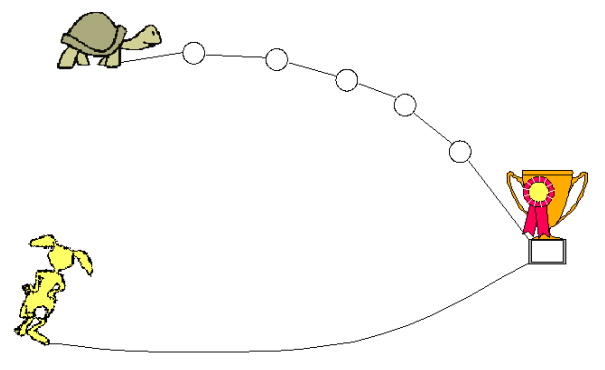
\includegraphics[width=0.5\textwidth]{image/lievre-tortue}
		\end{center}
		
	\subsection{Solution non orientée objet}
	%=======================================
	
		Pour ne pas aller trop vite et vous perdre tout de suite,
		commençons par une version non orientée objet du jeu.
		
		\subsubsection*{Représenter le jeu}
		%----------------------------------	

			Il faut d'abord se poser cette question :
			Comment représenter le jeu ?
			Une représentation du jeu doit être complète.
			C'est-à-dire qu'à partir de cette représentation,
			on doit pouvoir indiquer exactement où on en est dans le jeu
			et pouvoir le poursuivre.
			
			Pour le dire autrement, 
			imaginons qu'on joue à ce jeu \og{}en vrai\fg{}, sur une table de jeu.
			La représentation informatique doit capturer tout ce qui est pertinent
			dans le jeu physique de sorte que, si on range la boite de jeu,
			on peut, le lendemain, reconstruire le jeu exactement comme il était.
			
			Dans notre exemple, cela veut dire quoi ?
			\begin{description}
			\item[La tortue]
				On doit pouvoir savoir où elle en est dans son avancée.
				Un petit entier (de 0 à \nbMaxKmTortue{}) reprenant son avancée en km suffit.
				Appelons-le \lda{avancéeTortue} par exemple.
			\item[Le lièvre]
				Pendant le jeu, il est en permanence au départ
				et lorsque sort un 6, il atteint directement l'arrivée.
				Plusieurs possibilités s'offrent à nous :
			
				\begin{enumerate}
				\item
					On pourrait imaginer un entier valant 0 ou \nbMaxKmTortue{},
					appelé \lda{avancéeLièvre}.
				\item
					On pourrait aussi imaginer un booléen à vrai 
					lorsqu'il est au départ et faux lorsqu'il est à l'arrivée.
					On pourrait l'appeler \lda{lièvreAuDépart}.
				\item
					Ou encore un booléen ayant exactement le sens inverse.
					Le nom devra être choisi judicieusement pour ne pas induire
					le lecteur en erreur.
					Par exemple, ici, on pourrait choisir \lda{lièvreArrivé}.
				\end{enumerate}
				
				Ici, le troisième choix nous semble le plus pertinent.
			\item[Le dé]
				Un entier de 1 à 6 suffit pour représenter le résultat d'un dé.
				Appelons-le simplement \lda{dé}.
			\item[Les joueurs]
				Si on observe un jeu physique,
				on peut s'attarder sur les personnes en train de jouer.
				Faut-il les représenter ?
				On pourrait imaginer de connaitre leur nom,
				le nombre de fois qu'elles ont joué à ce jeu,
				leur nombre de victoires.
				Dans l'énoncé, 
				rien n'indique qu'il faille tenir compte de tout cela. 
				On s'intéresse au jeu proprement dit, et c'est tout.
			\item[Le plateau]
				On peut imaginer que dans le jeu physique,
				il y aurait une sorte de plateau 
				avec des km indiqués
				sur lequel avancerait la tortue.
				Mais il n'y a aucune information changeante
				sur ce plateau qui vaille la peine d'être retenue.
			\end{description}

		\subsubsection*{Un macro algorithme}
		%----------------------------------	
				
			Avant de se lancer dans l'écriture d'une solution détaillée du jeu,
			commençons par une solution non détaillée
			et voyons si tout semble clair et faisable.
			
			\begin{LDA}
				\Algo{jeuLièvreTortue}{}{}
					\Stmt Initialiser le jeu
					\While{le jeu n'est pas fini}
						\Stmt{Lancer le dé}
						\If{le dé est 6}
							\Stmt Le lièvre est arrivé
						\Else
							\Stmt La tortue avance
						\EndIf
						\Write l'état du jeu
					\EndWhile
					\Write le vainqueur
				\EndAlgo
			\end{LDA}
			
		\subsubsection*{Détailler l'algorithme}
		%----------------------------------	
	
			Repassons à présent sur l'algorithme
			et vérifions que nous pouvons détailler 
			chacun des points restés généraux.
			\begin{itemize}
			\item \textbf{Initialiser le jeu.}
				Il suffit de placer la tortue en 0
				et d'indiquer que le lièvre n'est pas encore arrivé.
				La valeur initiale du dé n'a pas d'importance.
			\item \textbf{Le jeu n'est pas fini.}
				Le jeu sera fini lorsque le lièvre sera arrivé
				(ce qu'on peut tester grâce au booléen \lda{lièvreArrivé})
				ou que la tortue sera au km \nbMaxKmTortue{}.
			\item \textbf{Lancer le dé.}
				C'est trivial si on utilise l'algorithme \lda{hasard()}
				à notre disposition.
			\item \textbf{Le lièvre est arrivé.}
				Il suffit de mettre le booléen \lda{lièvreArrivé} à vrai.
			\item \textbf{La tortue avance.}
				C'est trivial.
			\item \textbf{Afficher l'état du jeu.}
				À savoir, sur quelle face est tombé le dé
				et où se trouvent à présent le lièvre et la tortue.
			\item \textbf{Afficher le vainqueur.}
				Ce sera le lièvre si son booléen est à vrai et la tortue sinon
				(dans ce cas, son avancée sera forcément de \nbMaxKmTortue{} 
				puisque le jeu est fini).
			\end{itemize}

\clearpage		
			Au final, on obtient :
			\begin{LDA}
				\Algo{jeuLièvreTortue}{}{}
					\Decl{avancéeTortue}{entier}
					\Decl{lièvreArrivé}{booléen}
					\Decl{dé}{entier}

					\Empty
					\Let avancéeTortue \Gets 0
					\Let lièvreArrivé \Gets faux
					
					\Empty
					\While{avancéeTortue < \nbMaxKmTortue{} ET NON lièvreArrivé}
						\Let dé \Gets hasard(6)
						\If{dé = 6}
							\Let lièvreArrivé \Gets vrai
						\Else
							\Let avancéeTortue \Gets avancéeTortue + 1
						\EndIf
						\Write dé, avancéeTortue, lièvreArrivé
					\EndWhile

					\Empty
					\If{lièvreArrivé}
						\Write "Le lièvre a gagné"
					\Else
						\Write "Le tortue a gagné"
					\EndIf
				\EndAlgo
			\end{LDA}

	\subsection{Solution orientée objet}
	%=======================================
		
		Voyons à présent ce que ça pourrait donner si on introduit
		de l'orienté objet.
		Examinons d'abord les objets physiques du jeu.
		\begin{description}
		\item[La tortue]
			On peut envisager de définir une classe pour la tortue.
			Une tortue a une avancée. 
			Au départ, elle est au kilomètre 0.
			Elle peut avancer d'un kilomètre à la fois.
			Elle a fini et gagne lorsqu'elle arrive au kilomètre \nbMaxKmTortue{}.

			\begin{LDA}
				\Class{Tortue}
				\Private
					\Decl{avancée}{entier}
				\Public
					\Constr{Tortue}{}
						\Let avancée \Gets 0						
					\EndConstr
					\Empty
					\Method{avancer}{}{}
						\Let avancée \Gets avancée + 1						
					\EndMethod
					\Empty
					\Method{estArrivée}{}{booléen}
						\Return avancée = \nbMaxKmTortue{}
					\EndMethod
					\Empty
					\Method{getAvancée}{}{entier}
						\Return avancée
					\EndMethod
				\EndClass
			\end{LDA}

			Remarquez qu'on n'introduit pas de mutateur
			car on veut que la tortue n'avance qu'en respectant les
			règles du jeu.

		\item[Le lièvre]
			On peut appliquer la même démarche pour le lièvre
			qui aurait un attribut booléen indiquant s'il est arrivé ou pas.

		\item[Le dé]		
			Le dé est également un objet de notre jeu
			et peut être défini via une classe.

			\begin{minipage}{6cm}
			\begin{LDA}
				\Class{Lièvre}
				\Private
					\Decl{arrivé}{booléen}
				\Public
					\Constr{Lièvre}{}
						\Let arrivé \Gets faux					
					\EndConstr
					\Empty
					\Method{avancer}{}{}
						\Let arrivé \Gets vrai
					\EndMethod
					\Empty
					\Method{estArrivé}{}{booléen}
						\Return arrivé
					\EndMethod
				\EndClass
			\end{LDA}
			\end{minipage}
			~
			\begin{minipage}{6cm}
			\begin{LDA}
				\Class{Dé}
				\Private
					\Decl{valeur}{entier}
				\Public
					\Constr{Dé}{}
					\EndConstr
					\Empty
					\Method{lancer}{}{}
						\Let valeur \Gets hasard(6)
					\EndMethod
					\Empty
					\Method{getValeur}{}{entier}
						\Return valeur
					\EndMethod
				\EndClass
			\end{LDA}
			\end{minipage}

		\end{description}

		\subsubsection*{L'algorithme du jeu}
		%-----------------------------------
		
			L'algorithme du jeu peut être récrit
			en utilisant les trois classes qu'on vient de définir.
			
			\begin{LDA}
				\Algo{jeuLièvreTortue}{}{}
					\Decl{tortue}{Tortue}
					\Decl{lièvre}{Lièvre}
					\Decl{dé}{Dé}

					\Empty
					\Let tortue \Gets \K{nouvelle} Tortue()
					\Let lièvre \Gets \K{nouveau} Lièvre()
					\Let dé \Gets \K{nouveau} Dé()
					
					\Empty
					\While{NON tortue.estArrivée() ET NON lièvre.estArrivé()}
						\Stmt dé.lancer()
						\If{dé.getValeur()=6}
							\Stmt lièvre.avancer()
						\Else
							\Stmt tortue.avancer()
						\EndIf
						\Write dé.getValeur(), tortue.getAvancée(), lièvre.estArrivé()
					\EndWhile

					\Empty
					\If{lièvre.estArrivé()}
						\Write "Le lièvre a gagné"
					\Else
						\Write "Le tortue a gagné"
					\EndIf
				\EndAlgo
			\end{LDA}
			
			Est-ce une bonne idée d'avoir défini ces trois classes ?
			C'est une question qu'il est légitime de se poser
			quand les classes sont aussi simples.
			Remarquons toutefois que le code est plus modulaire
			et que la méthode principale est plus facile à lire.
			
			La classe \lda{Dé} se justifie d'autant plus 
			qu'elle pourra probablement servir à de nombreuses occasions.
			Ce sera encore plus le cas
			si on la généralise à des dés qui n'ont pas forcément 6 faces.

			\begin{LDA}
				\Class{Dé}
				\Private
					\Decl{nbFaces}{entier}
					\Decl{valeur}{entier}
				\Public
					\Constr{Dé}{\Par{nf}{entier}}
						\Let nbFaces \Gets nf
					\EndConstr
					\Empty
					\Method{lancer}{}{}
						\Let valeur \Gets hasard(nbFaces)
					\EndMethod
					\Empty
					\Method{getValeur}{}{entier}
						\Return valeur
					\EndMethod
				\EndClass
			\end{LDA}
			
			Dans l'algorithme principal,
			le seul changement est la création du dé qui devient :
			\begin{LDA}
					\Let dé \Gets \K{nouveau} Dé(6)
			\end{LDA}
				
	\subsection{Solution MVC (\og{}Modèle-Vue-Contrôleur\fg{})}
	%=======================================
		
		Dans la version OO qu'on vient de voir,
		on a introduit trois classes 
		mais il reste tout un morceau, l'algorithme principal, qui n'est pas OO.
		Peut-on aller plus loin dans l'OO ?
		Bien sûr ! 
		Mais il y a de bonnes et de mauvaises façons de le faire.
		
		La mauvaise approche 
		est de simplement mettre l'algorithme principal dans une classe.
		Ce qui donnerait :

		\begin{LDA}
			\Class{LièvreTortue}
				\Constr{LièvreTortue}{}
				\EndConstr
				\Empty
				\Method{jouer}{}{}
					\LComment Idem algorithme jeuLièvreTortue() ci-avant  
				\EndMethod
			\EndClass
		\end{LDA}
		
		Ce qui réduirait l'algorithme principal à :
		\begin{LDA}
			\Algo{jeuLièvreTortue}{}{}
				\Decl{jeu}{LièvreTortue}
				\Let jeu \Gets \K{nouveau} LièvreTortue()
				\Stmt jeu.jouer()
			\EndAlgo
		\end{LDA}
		ou même, en se passant de la variable locale :
		\begin{LDA}
			\Algo{jeuLièvreTortue}{}{}
				\Stmt (\K{nouveau} LièvreTortue()).jouer()
			\EndAlgo
		\end{LDA}

		Cette approche est correcte mais n'exploite en rien 
		les avantages de l'OO.
		Une meilleure idée est de suivre l'approche MVC
		que nous allons vous expliquer.
		
		Dans l'approche MVC,
		on découpe le code en différentes parties.
		La partie \og{}modèle\fg{} regroupe les bouts de code
		qui font vraiment quelque chose (on parle de \og{}métier\fg{})
		tandis que la partie \og{}vue\fg{} regroupe les bouts de code
		qui interagissent avec l'utilisateur (demandes et affichages).
		La partie \og{}contrôleur\fg{}, quant à elle,
		conserve le code qui fait le lien entre le modèle et la vue.
		
		Si on respecte cette approche, 
		le métier ne contient \textbf{aucune} interaction avec l'utilisateur
		et la vue ne s'occupe \textbf{que} de l'interaction avec l'utilisateur.
		Il y a là de nombreux avantages :
		\begin{itemize}
		\item
			Les compétences pour écrire le modèle
			(connaissance du métier, accès à des bases de données\dots)
			et le dialogue avec les utilisateurs 
			(ergonomie, graphisme\dots)
			ne sont pas les mêmes.
			On peut donc confier ces parties à des équipes spécialisées.
		\item
			On pourra facilement changer le dialogue avec l'utilisateur.
			Ainsi, si on possède une version console du jeu,
			il suffira, pour en faire une autre version 
			(console, graphique, web\dots)
			de recommencer la vue 
			(et probablement d'adapter le contrôleur)
			sans toucher au modèle.
		\end{itemize}
	
		\paragraph{Le modèle.}
		%---------------------
		Dans notre exemple, le modèle contiendrait les algorithmes suivants :
		\begin{itemize}
		\item
			Initialiser le jeu : 
			placer la tortue et le lièvre à leur position de départ.
		\item
			Jouer un coup : 
			lancer le dé et déplacer le lièvre ou la tortue.
		\item
			Tester si le jeu est fini ou pas.
		\item
			Trouver le vainqueur.
		\end{itemize}

		Chacun de ces algorithmes est implémenté par une méthode
		(sauf l'initialisation qui est du ressort du constructeur).
		Au niveau des attributs, 
		on retrouve les éléments du jeu : le lièvre, la tortue et le dé.
		\footnote{%
			Une autre façon de voir les choses
			est de dire qu'on trouve en attributs
			les variables locales de la version non OO
			qui sont partagées par les différentes méthodes.
			Ici, il s'agit de toutes les variables locales
			mais ce n'est pas toujours le cas.
			Le dé, par exemple, n'est un attribut que parce que
			la vue voudra le connaitre pour le montrer à l'utilisateur.
			Sans cela, il pourrait être une variable locale
			de la méthode \lda{jouerCoup()}.
		}
		
		Ce qui donne :
		\begin{LDA}
			\Class{LièvreTortue}
				\Private
					\Decl{tortue}{Tortue}
					\Decl{lièvre}{Lièvre}
					\Decl{dé}{Dé}
				\Public
					\ConstrSign{LièvreTortue}{}
					\MethodSign{estFini}{}{booléen}
					\MethodSign{jouerCoup}{}{}
					\MethodSign{getVainqueur}{}{chaine}
					\LComment
						+ les accesseurs (getLièvre(), getTortue() et getDé())
						des attributs mais pas les mutateurs
			\EndClass
		\end{LDA}
		
		\begin{LDA}
			\Constr{LièvreTortue}{}
				\Let tortue \Gets \K{nouvelle} Tortue()
				\Let lièvre \Gets \K{nouveau} Lièvre()
				\Let dé \Gets \K{nouveau} Dé(6)						
			\EndConstr				
			\Empty
			\Method{estFini}{}{booléen}
				\Return tortue.estArrivée() OU lièvre.estArrivé()
			\EndMethod
		\end{LDA}
		
		\begin{LDA}
			\Method{jouerCoup}{}{}
				\Stmt dé.lancer()
				\If{dé.getValeur()=6}
					\Stmt lièvre.avancer()
				\Else
					\Stmt tortue.avancer()
				\EndIf
			\EndMethod

			\Empty
			\Method{getVainqueur}{}{chaine}
				\If{lièvre.estArrivé()}
					\Return "Lièvre"
				\ElsIf{tortue.estArrivée()}
					\Return "Tortue"
				\Else
					\Return "Aucun, partie en cours"
				\EndIf
			\EndMethod
		\end{LDA}
			
		Remarque : Dans un langage comme \bsc{Java}, la méthode 
		\lda{getVainqueur()} pourrait lancer une \texttt{IllegalStateException}
		si elle est appelée avant que la partie ne soit finie.
		
		\paragraph{La vue.}
		%---------------------
		Avec notre exemple, plutôt simple, il n'y a pas de lecture
		mais il reste des affichages :
		\begin{itemize}
		\item
			Afficher l'état du jeu après un coup : 
			valeur du dé et nouvelles positions du lièvre et de la tortue.
		\item
			Afficher le vainqueur.
		\end{itemize}
		
		Cet exemple est probablement trop simple pour nécessiter une classe%
		\footnote{
			Une erreur classique est de placer ces algorithmes
			dans les classes associées du modèle
			car cela contrevient à la règle : 
			aucune interaction utilisateur dans le modèle.
		}.
		On pourrait se contenter de deux algorithmes classiques.
		
		\begin{LDA}
			\Algo{afficherÉtat}{\Par{jeu}{LièvreTortue}}{}
				\Write jeu.getDé().getValeur()
				\Write jeu.getTortue().getAvancée()
				\Write jeu.getLièvre().estArrivé()
			\EndAlgo
			
			\Empty
			\Algo{afficherVainqueur}{\Par{jeu}{LièvreTortue}}{}
				\Write "Le gagnant est : ", jeu.getVainqueur()
			\EndAlgo
		\end{LDA}
		
		\paragraph{Le contrôleur.}
		%-------------------------
		
		Le contrôleur est ce qui n'a pas été placé dans la vue ou le modèle,
		c'est-à-dire le code qui crée la dynamique entre tous ces éléments.

		\begin{LDA}
			\Algo{jeuLièvreTortue}{}{}
				\Decl{jeu}{LièvreTortue}
				\Stmt jeu \Gets \K{nouveau} LièvreTortue()
				\While{NON jeu.estFini()}
					\Stmt jeu.jouerCoup()
					\Stmt afficherÉtat(jeu)
				\EndWhile
				\Stmt afficherVainqueur(jeu)
			\EndAlgo
		\end{LDA}
		
		Remarquez la concision et la lisibilité de ce qu'on vient d'écrire.
